\begin{figure}
\begin{center}
\resizebox{\columnwidth}{!}{
\begin{tabular}{ccc}
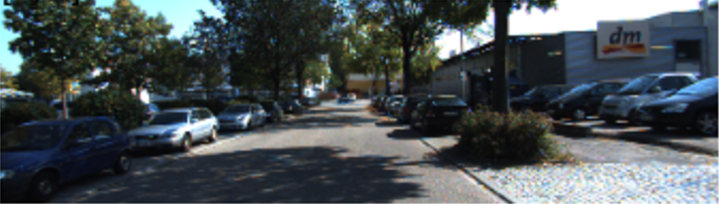
\includegraphics[width=0.5\textwidth]{./figs/fcn_out/fcn_input.png} &
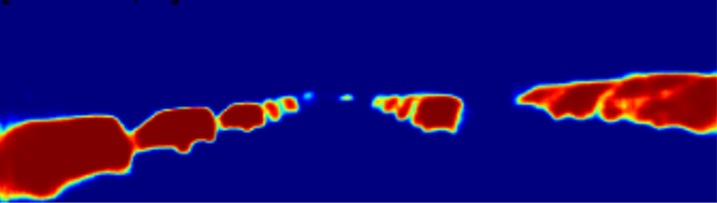
\includegraphics[width=0.5\textwidth]{./figs/fcn_out/fcn_seg.png} &
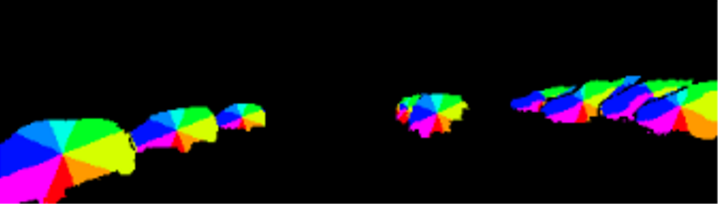
\includegraphics[width=0.5\textwidth]{./figs/fcn_out/fcn_angle.png}
\end{tabular}
}
\caption{Illustration of the output of the pretrained FCN. Left: input image.
Middle: predicted foreground. Right: predicted angle map.}
\label{fig:fcn}
\end{center}
\end{figure}
